%! TEX root = ../main.tex
\documentclass[../main]{subfiles}

\begin{document}
\chapter{部誌を作る} % タイトル
\rightline{4年 森山 陽介} % 学年と名前(ハンドルネームでも可)
部誌を作るためには何が必要か。\par
それはPDFを結合、分解、編集できることです。\par
そのためなら、究極的には何でもよくて、Adobe AcrobatやAdobe InDesignなんかを使ってもいいでしょう。ただ、有料だし、一時的に担当する部誌のために自腹を切るのも、部費を使うのも割にあわないでしょう。どうせなら、今後の学生生活にも役立つようなスキルを身に着けられるような作業にもしたいものです。\par
そこで、部誌の作成に当たっては{\LaTeX}を使用することにしました。特に、この部誌で使用する{Lua\LaTeX}は、フォントを変更するのが容易ですし、{(u)p\LaTeX}で必要になるようなdvipdfmxやそのオプションを必要とせずに直接PDF化でき、今後主流となるようなモダンなエンジンと言われています。\footnote{ここは単に思想というか、こだわりに近い}記事も{\LaTeX}で書けるので、そうすればPDF化も1回で済むし、体裁は勝手にやってくれるので作業量を減らすことができます。\footnote{{\LaTeX}自体の体裁がなってない原稿を手直しする手間やエラー対応はあるけどね。}\par
一方で、表紙や裏表紙など、グラフィックなデザインは{\LaTeX}くんの得意とするところではないので、人間が作る必要があります。こういったときに使用するのは、ベクターグラフィックス\footnote{コンリテで習いましたよね?}を扱えるソフトです。一般的に有名なのはAdobe Illustratorでしょうが、これまた有料だし、Illustratorで作ったファイルはPDF化しない限りIllustratorでしか開けないので、引き継ぎやすさに難があります。ここでは、フリーでWindoows, Mac, Linux全てに対応しているInkscapeというソフトを用いて、グラフィカルなページのデザインを行います。
\section{\LaTeX 環境構築とその準備}
\LaTeX 環境を構築しましょう。おそらくほとんどの電通大生なら自分のマシンにインストールなりされてると思いますが、それぞれマシンも違えば、使用してる\TeX エンジンも異なるでしょう。違う環境で同じファイルを扱うとどこかで齟齬が生じるので、Dockerを使って、仮想環境を用意して、そこで部誌を編集することにしてみました。基本的には\url{https://zenn.dev/being/articles/how-to-use-my-latex}の内容を基に環境構築したので、この通りにすればできるはず。一応、必要なことをサンプルがてら書いておきます。

\subsection{必要なもの}
\begin{itemize}
  \item VScode
  \item Docker Desktop
  \item Git
  \item GitHubアカウント
  \item (WSL)
\end{itemize}
\subsection{Docker Desktopのインストール}
\url{https://www.docker.com/products/docker-desktop/}にアクセスして、Docker Desktopをインストールして、アカウント作成(飛ばしてもよい)など設定して起動させておきます。
\subsection{gitの準備}
gitをインストールするなりして、githubと連携できるようにします。\footnote{正直まだ良くわかってない部分も多くてちゃんと説明できる自信はない}
gitのインストールはWindowsだと面倒なので、Windowsの場合はWSL(Windows Subsystem for Linux)を利用します。Windows上にLinuxのUbuntu\footnote{好みのLinuxがある人はこの限りでない}を構築して操作するものです。初めての人は、Windowsの設定から「アプリ」$\rightarrow$「オプション機能」と進んで、一番下までスクロールしたところにある「Windowsのその他の機能」を選択します。そこに「Linux用Windowsサブシステム」の項目があるので、チャックボックスにチェックが入っているか確認してください。(\figref{wsl})入ってなかったら入れましょう。
\begin{figure}[H]
  \centering
  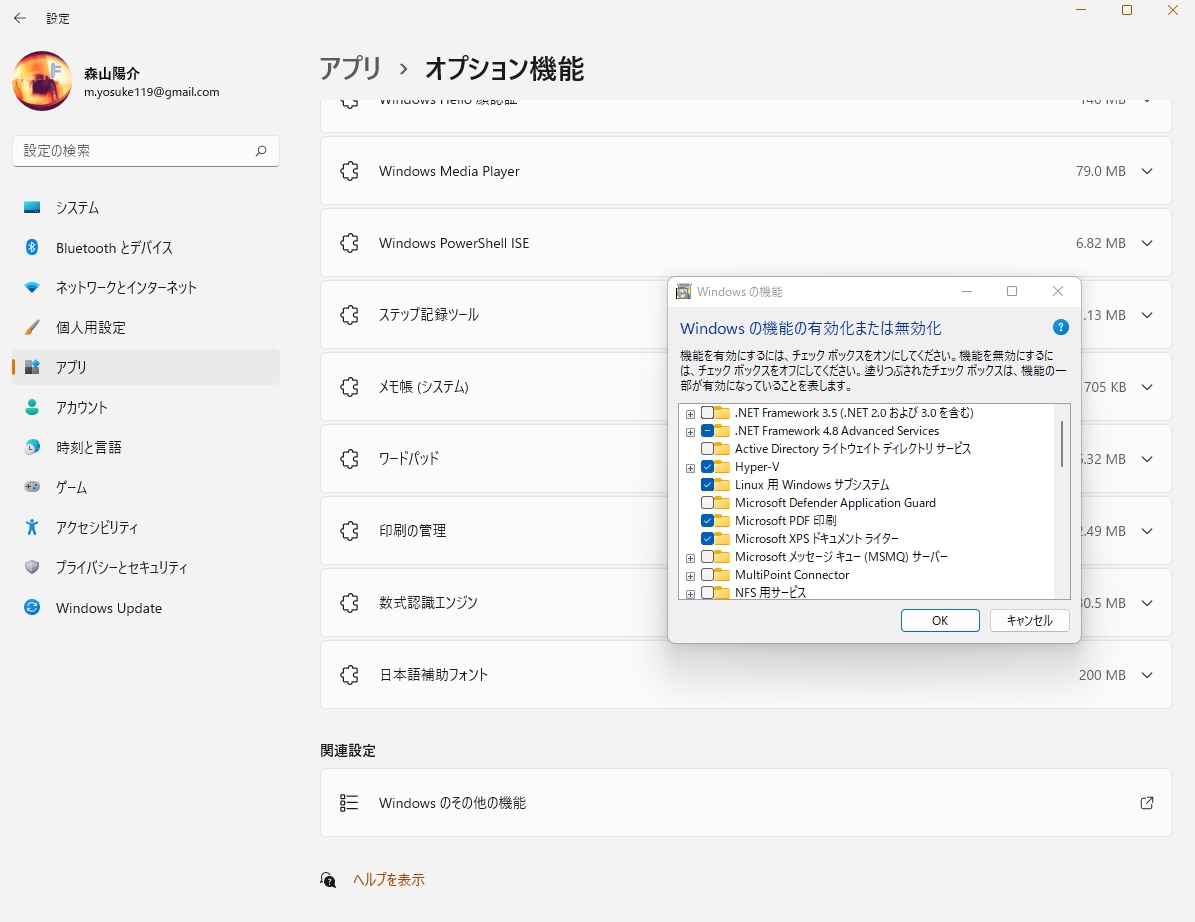
\includegraphics[width=.5\textwidth]{figures/ss274.png}
  \caption{WSLをインストールする準備}
  \label{fig:wsl}
\end{figure}
次に、PowerShellを管理者として開いて
\begin{lstlisting}
wsl --install
\end{lstlisting}
を入力して実行します。

すると、WSLがインストールされるので、WSLのターミナル画面を開いて、アカウント設定なり済ませて、
\begin{lstlisting}
sudo apt update
sudo apt upgrade
\end{lstlisting}
など済ませれば、gitはWSL内では使えるようになってるはず。なってなかったら
\begin{lstlisting}
sudo apt install git
\end{lstlisting}
とかすれば大丈夫だと思います。多分。

そしたら、GitHub(\url{https://github.com/})のアカウントを用意して、その情報をgitに設定しておきます。これを「gitの初期設定」と呼ばれているのをよく目にして最初は難のことやらさっぱりでした。
\begin{lstlisting}
git config --global user.name "GitHubアカウント名"
git config --global user.email GitHubに登録したメアド
git config --global code.editor 'code --wait' ← VScodeの場合
\end{lstlisting}
\subsection{VScodeの準備}
VScodeのDevContainerという機能を使って行うのが便利なので、それを推奨します。VScodeをインストールして、"Remort Development"という4つの拡張機能のパックとDockerの拡張機能をインストール。あとGitHubのアカウントとの連携とかしておきましょう。
\subsection{\LaTeX 環境構築}
WSLのターミナル上で、
\begin{lstlisting}
  docker pull ghcr.io/being24/latex-docker:latest
\end{lstlisting}
を実行したら、天文部GitHubにある(はず)の部誌用のファイル群をルートディレクトリごとclone($\risingdotseq$全部ダウンロード)してしまえば8割方完了です。

あとはそのディレクトリを(仮にWORKDIRとして)
\begin{lstlisting}
code WORKDIR
\end{lstlisting}
といったふうにVScodeで開いて、画面右下に出てくる「コンテナーで再度開く」をOKすれば、自動で環境構築が始まります。あとは画面の指示にイエスマンで従っていけば、完成です。多分。

\section{Inkscapeで表紙を作る}
Inkscape(\url{https://inkscape.org/ja/})をダウンロードして、新規作成でA4用紙を選択します。そして、表紙にしたい画像を選んで配置します。
\begin{figure}[H]
  \centering
  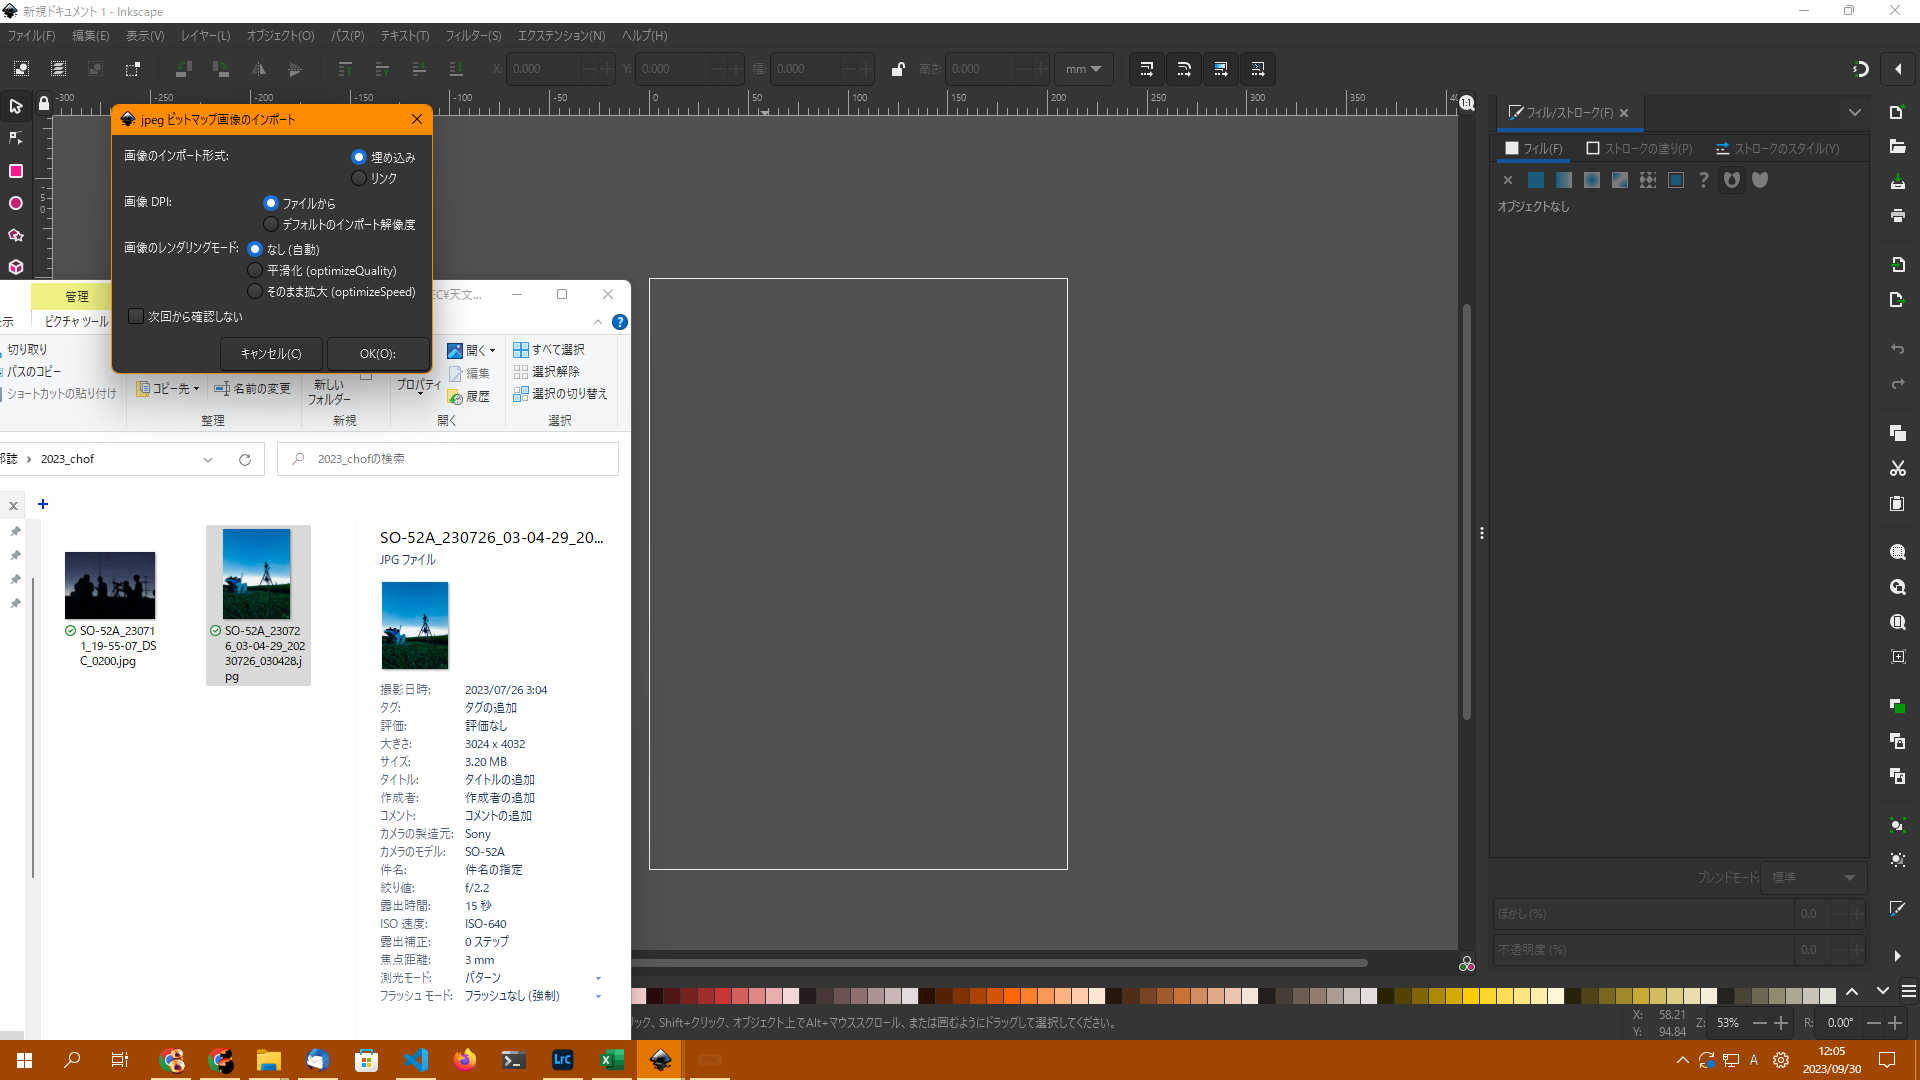
\includegraphics[width=.5\textwidth]{figures/ss265.png}
  \caption{表紙にしたい画像をドラッグ・アンド・ドロップ}
  \label{fig:ss265}
\end{figure}
画像の縦横比をロックした上で、幅を210にするか、高さを298にするかして、A4用紙にフィットさせます。そしたら、部誌タイトルの素材を同じくドラッグ・アンド・ドロップしていい感じの大きさと場所に配置します。\footnote{大きさと座標の数値を決められると自動化できそう}このとき、「ドキュメントのプロパティ」からグリッドを作成しておくと、配置するときの目印になって便利です。
\begin{figure}[H]
  \centering
  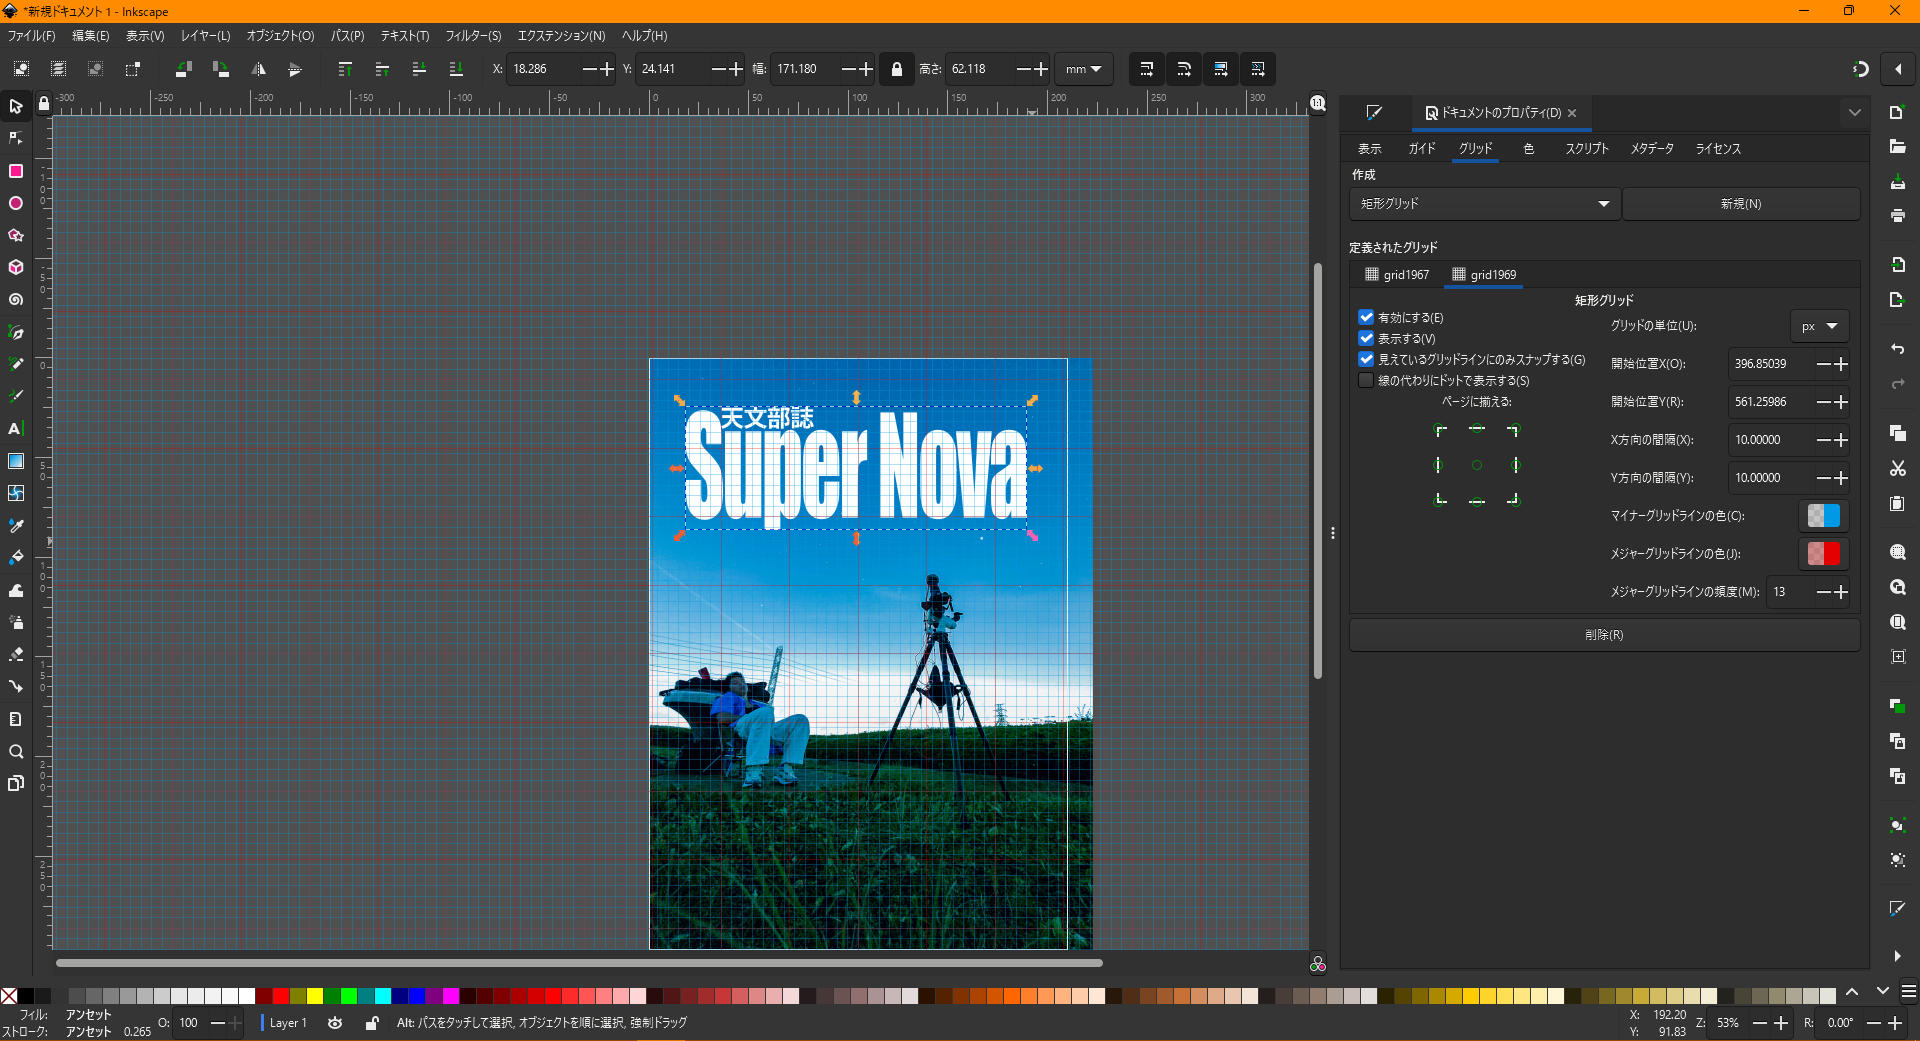
\includegraphics[width=.5\textwidth]{figures/ss267.png}
  \caption{タイトルの配置}
  \label{fig:ss267}
\end{figure}
あとは、目次に沿って注目タイトルをテキスト入れするとかクレジットを入れるとかして、表紙っぽくします。一通りできたら、「名前をつけて保存」でSVGファイルとして保存します。

微調整など繰り返して、ようやく表紙として完成したら、上書き保存はもちろんとして、「コピーを保存」からPDFを選択して、PDFとして出力します。
\begin{figure}[H]
  \centering
  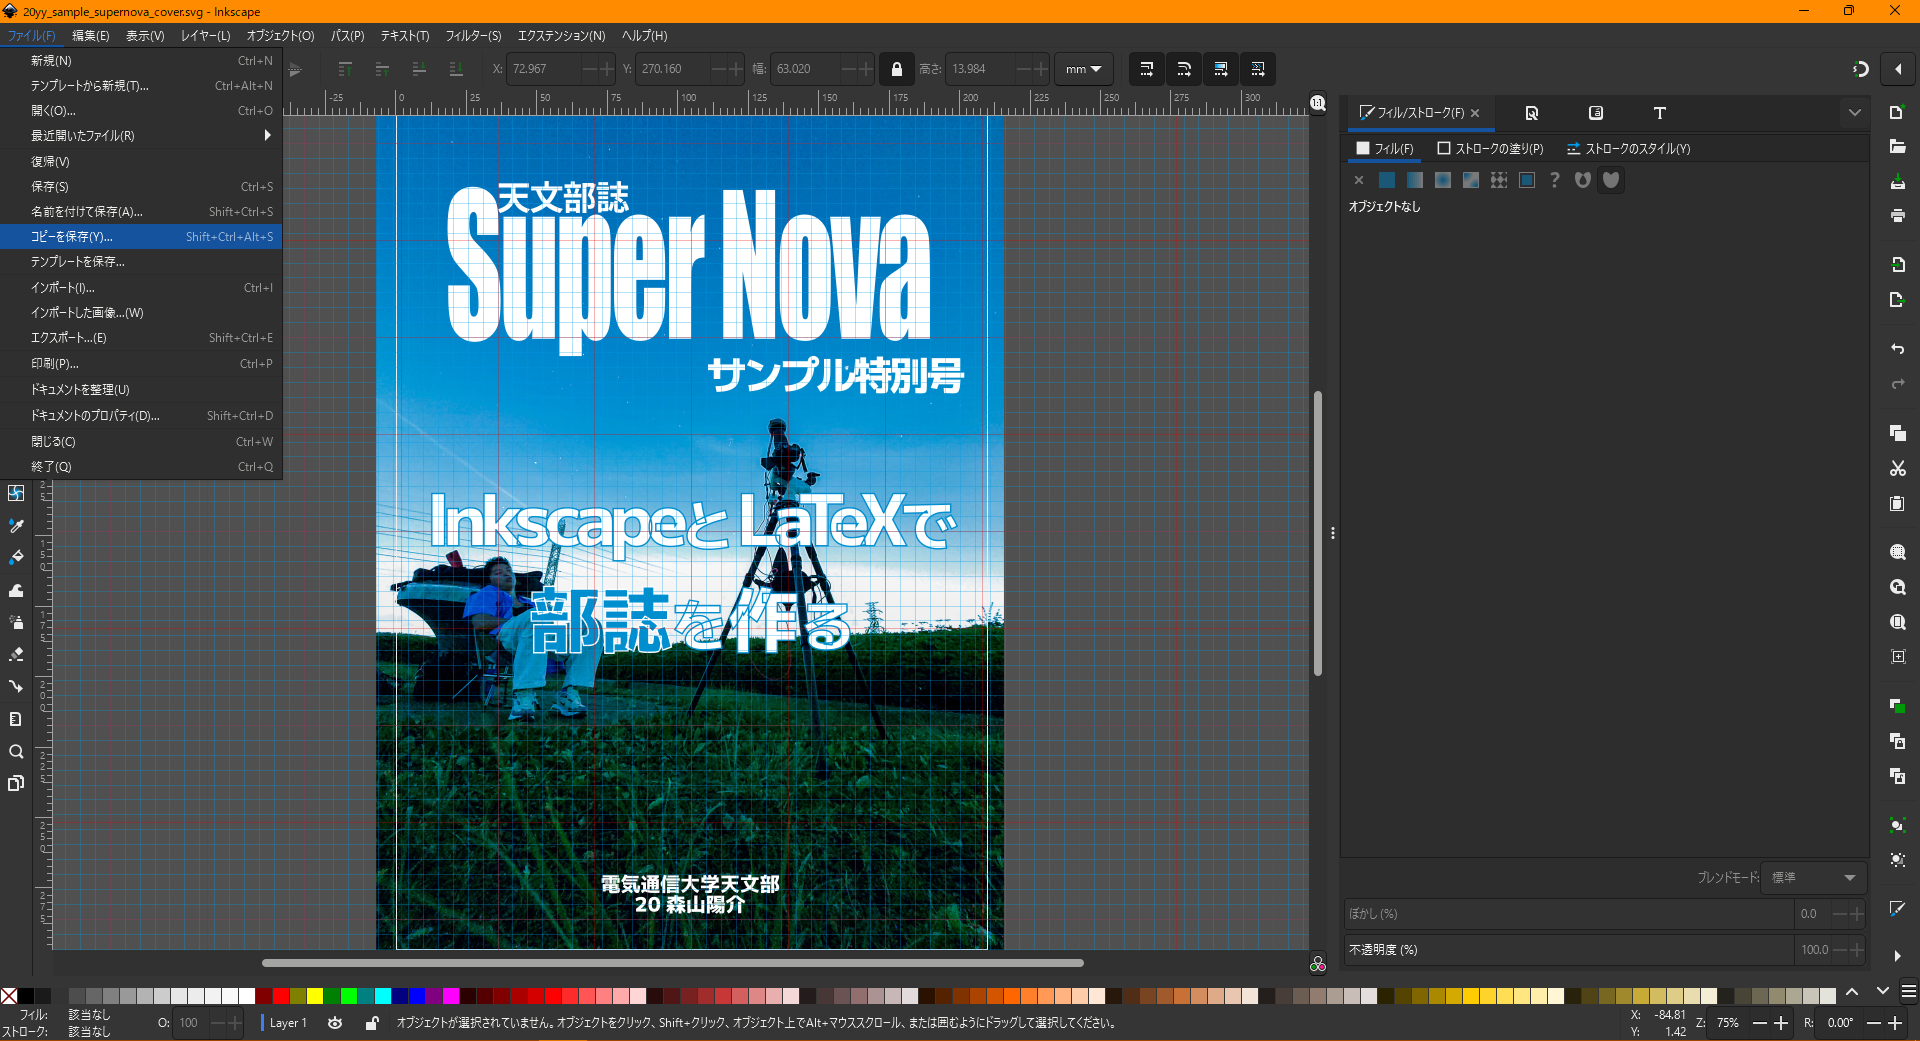
\includegraphics[width=.5\textwidth]{figures/ss270.png}
  \caption{コピーを保存}
  \label{fig:ss270}
\end{figure}
\begin{figure}[H]
  \centering
  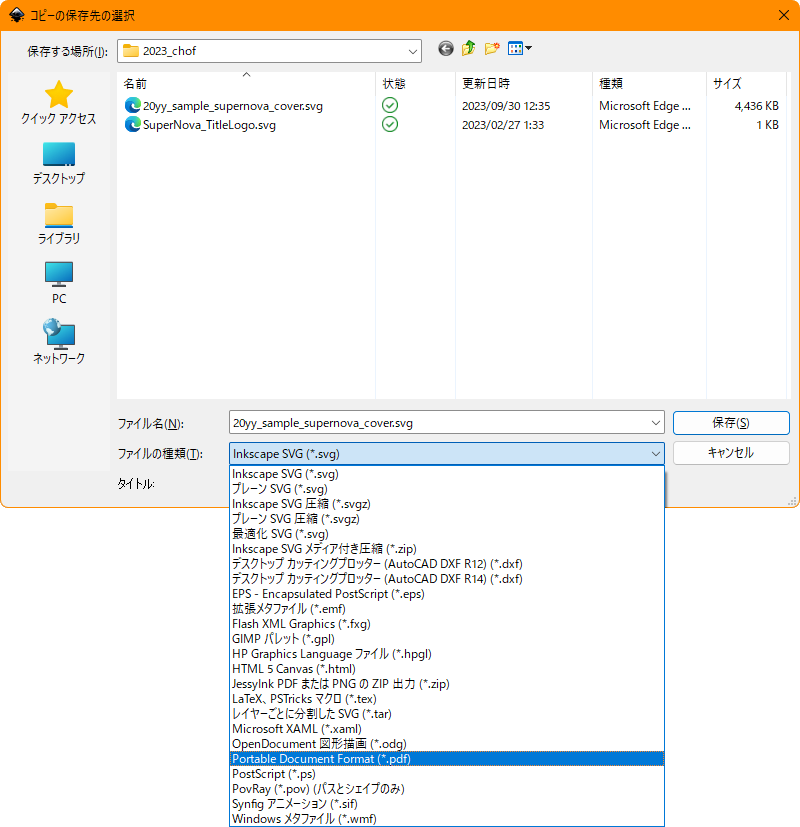
\includegraphics[width=.5\textwidth]{figures/ss272.png}
  \caption{Portable Document Format(PDF)を選択}
  \label{fig:ss272}
\end{figure}
\begin{figure}[H]
  \centering
  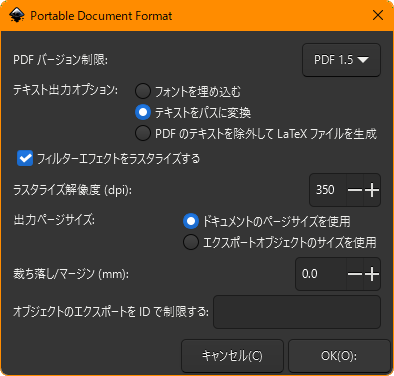
\includegraphics[width=.5\textwidth]{figures/ss273.png}
  \caption{PDFの出力設定}
  \label{fig:ss273}
\end{figure}
裏表紙も、同じようにして作ってしまえばOK!簡単でしょ?

\end{document}
